\documentclass[12pt]{article}
\usepackage[english]{babel}

\usepackage[a4paper,top=2cm,bottom=2cm,left=3cm,right=3cm,marginparwidth=1.75cm]{geometry}

% Useful packages
\usepackage{amsmath}
\usepackage{graphicx}
\usepackage[colorlinks=true, allcolors=blue]{hyperref}
\usepackage{enumitem}

\usepackage{natbib}



\title{Discipline name: Introduction to IoT and Cloud Architectures}
\author{Bârsan Patricia-Diana, Christian Cezara-Cala}

\begin{document}

% \textbf{Smart Garden Irrigation System} where soil moisture level is monitored using sensors and a water pump is controlled for irrigation.

\begin{figure}
\centering

\includegraphics[width=0.8\linewidth]{images/image5.png}
\end{figure}

\maketitle

\newpage

\section{Main features of the project}

\begin{itemize}[leftmargin=2cm]
    \item Data collection phase
    \item[] Through an Android application, the user activates a script, from a raspberrypi computer, that captures a picture of the plant with a webcam and triggers the dht and soil moisture sensors to collect data from the soil of the plant. An AI model is also used to identify the plant species. \\
    All the data is collected and sent to the AWS database and also back to the application, where it is displayed, along with a calculated watering routine based on the species of the identified plant. 
    \item Watering phase
    \item[] The user decides whether to water the plant using the recommended number and duration of pumps, or is free to modify them, and then another script is activated that controls the water pump to water the plant accordingly. 
    \item Extra
    \item[] All the data collected is displayed on a Flask website, separated by plant, along with a graph to show the evolution of the humidity and temperature of the soil of the plants as time passes.
\end{itemize}

\newpage

\section{Photos and screenshots of the project}
\subsection{Physical part}

\begin{figure}[ht]
    \centering
    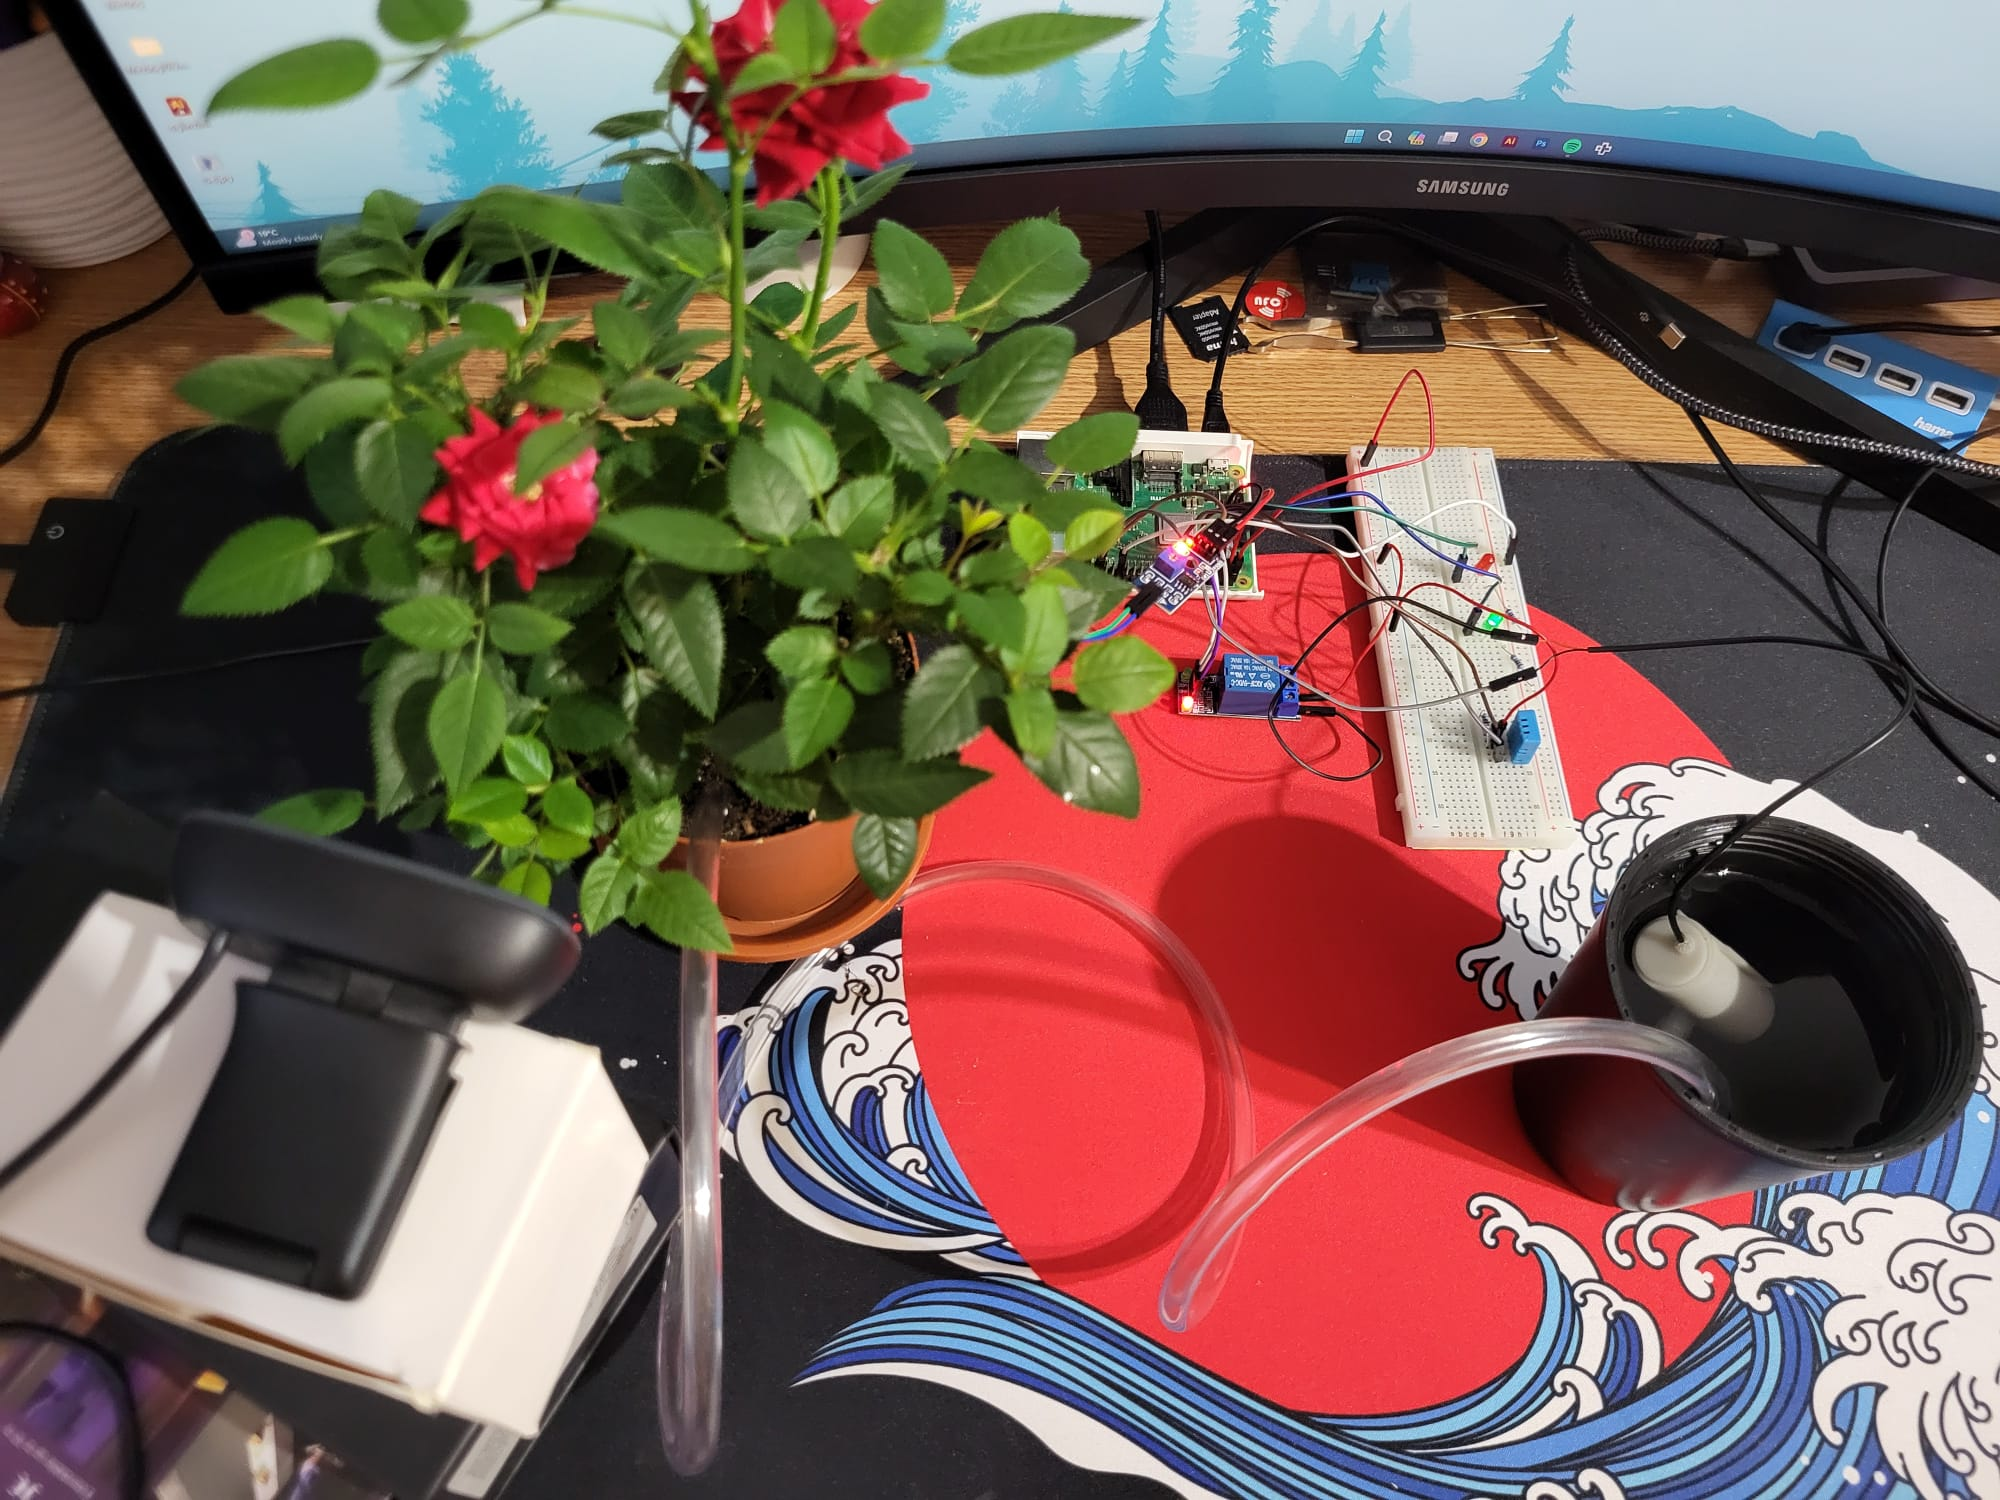
\includegraphics[width=1\textwidth]{images/image13.jpeg}
\end{figure} 

\begin{figure}[ht]
    \centering
    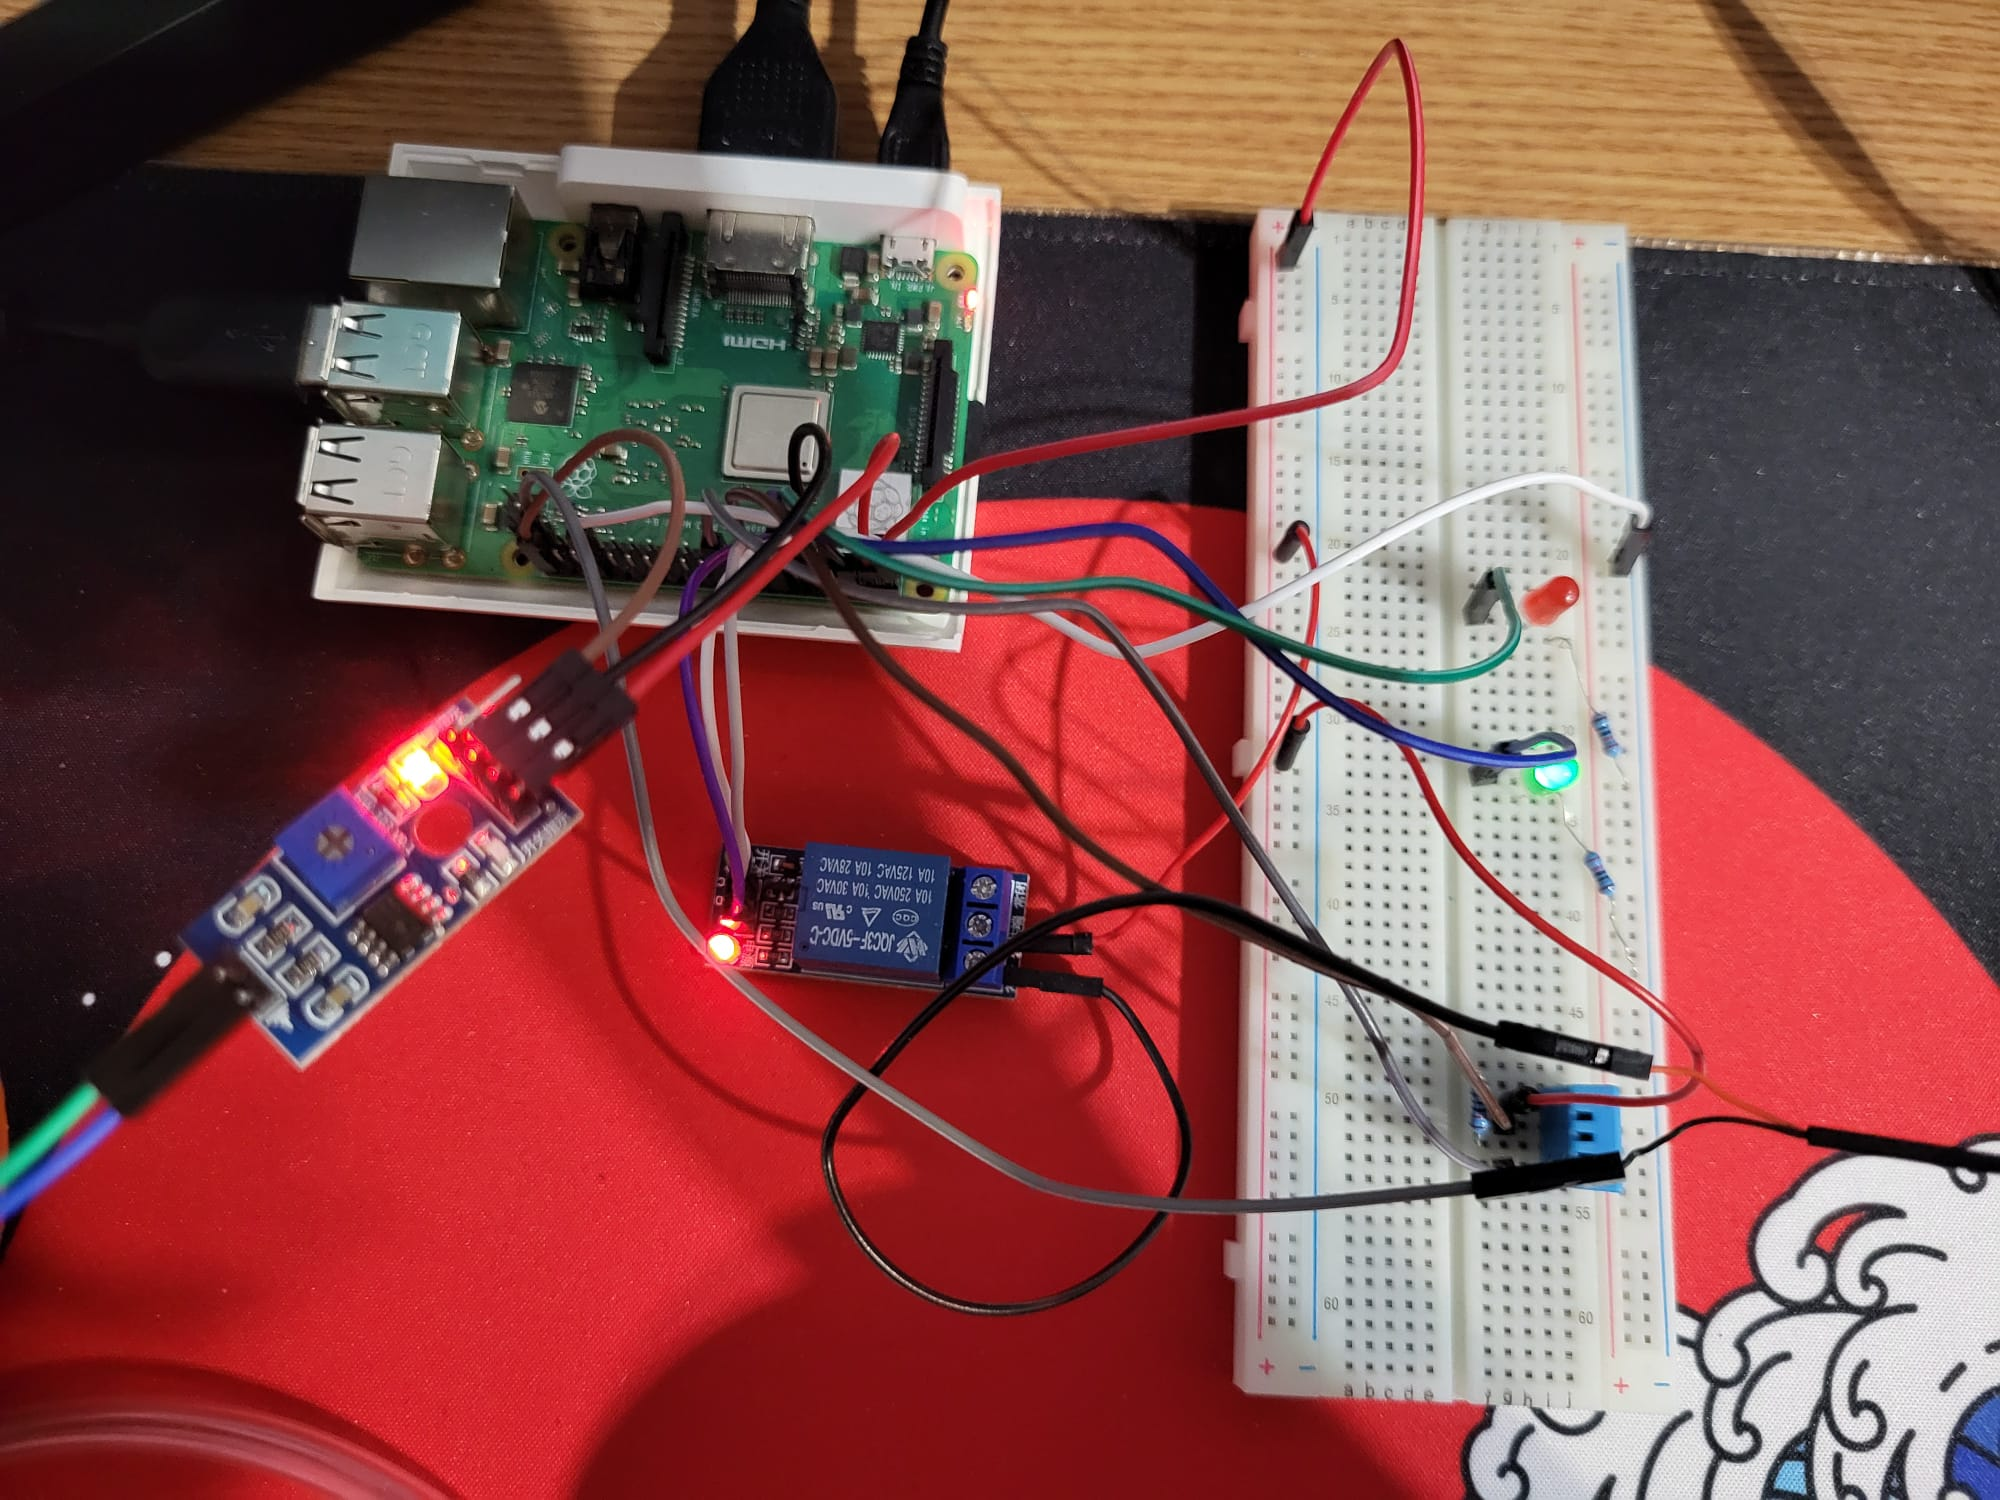
\includegraphics[width=0.65\textwidth]{images/image14.jpeg}
\end{figure} 

\newpage

\begin{figure}[ht]
    \centering
    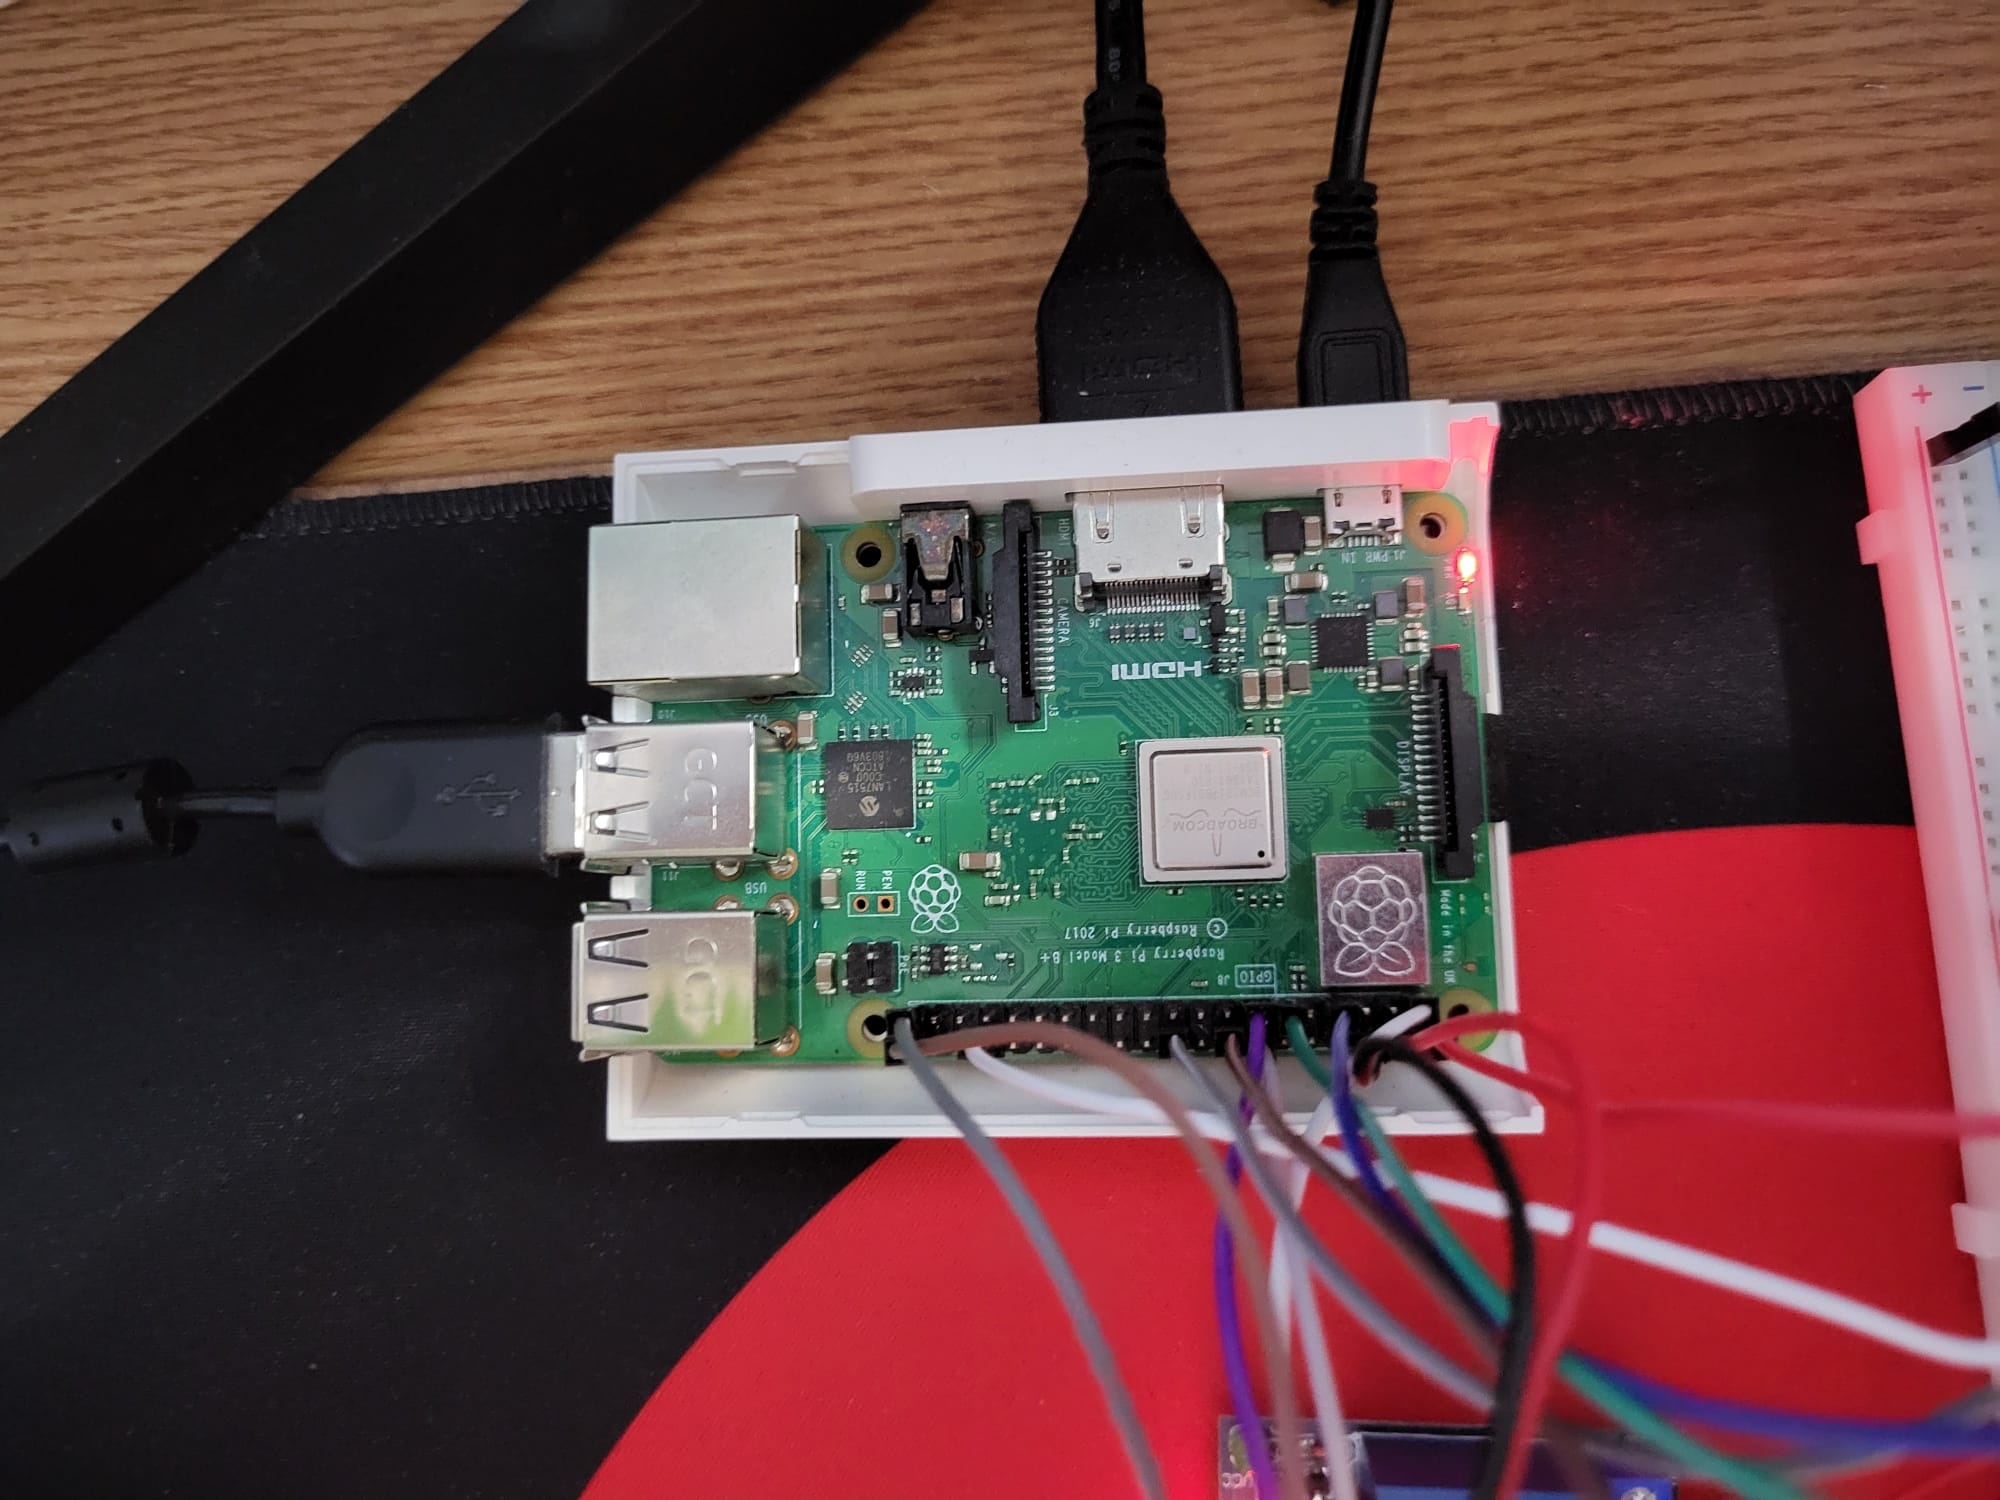
\includegraphics[width=0.53\textwidth]{images/image15.jpeg}
\end{figure} 

\begin{figure}[ht]
    \centering
    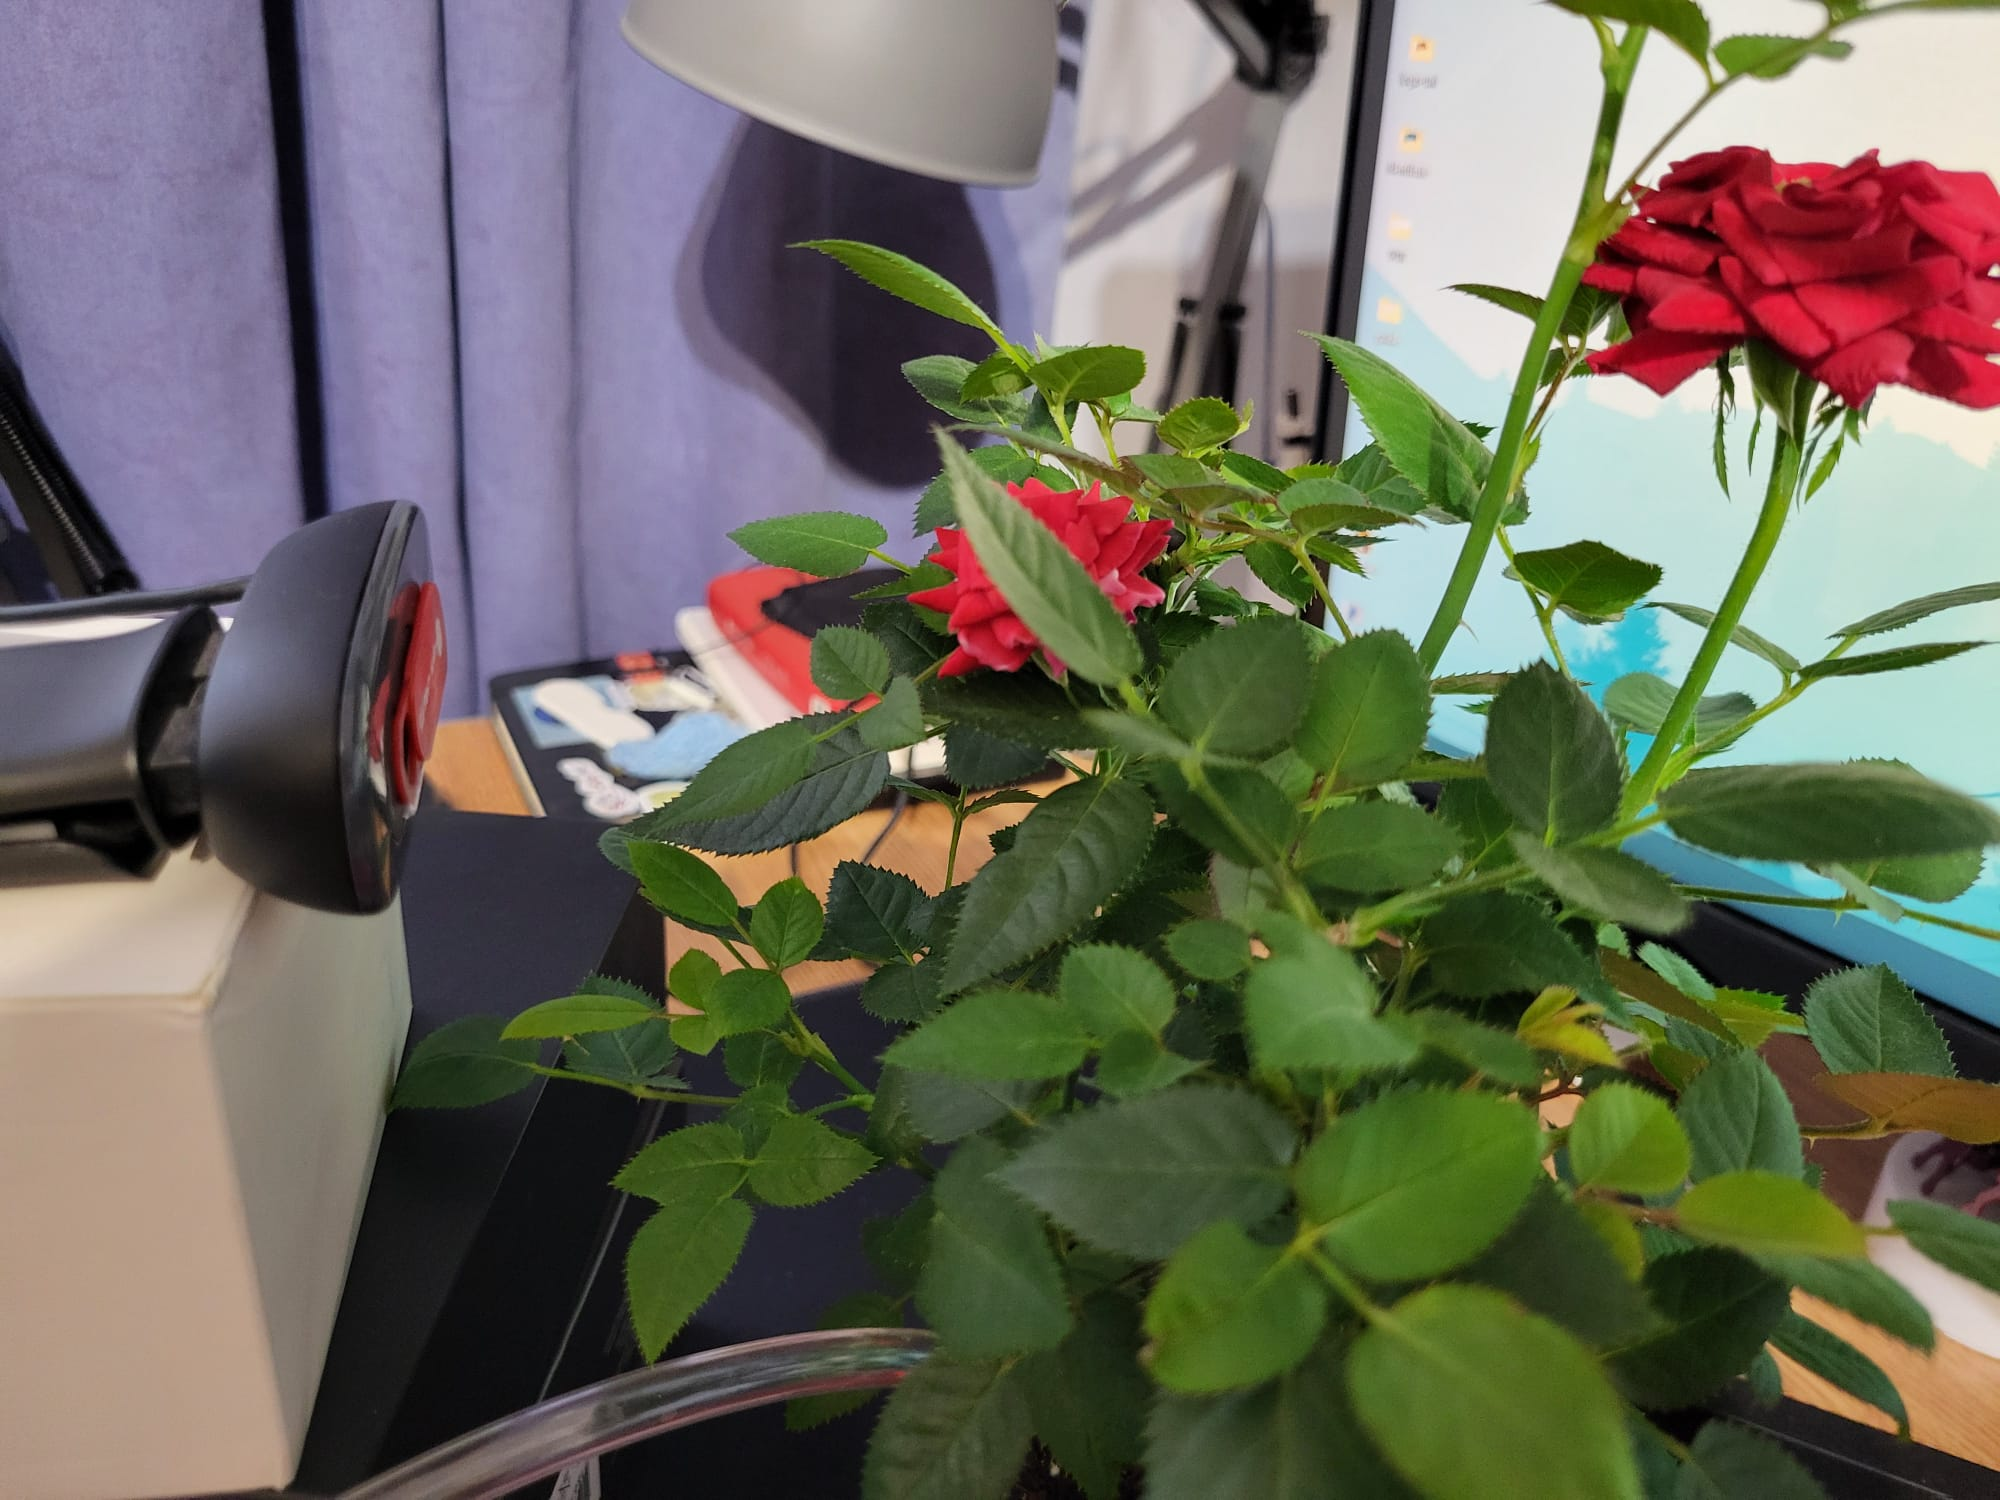
\includegraphics[width=0.53\textwidth]{images/image16.jpeg}
\end{figure} 

\begin{figure}[ht]
    \centering
    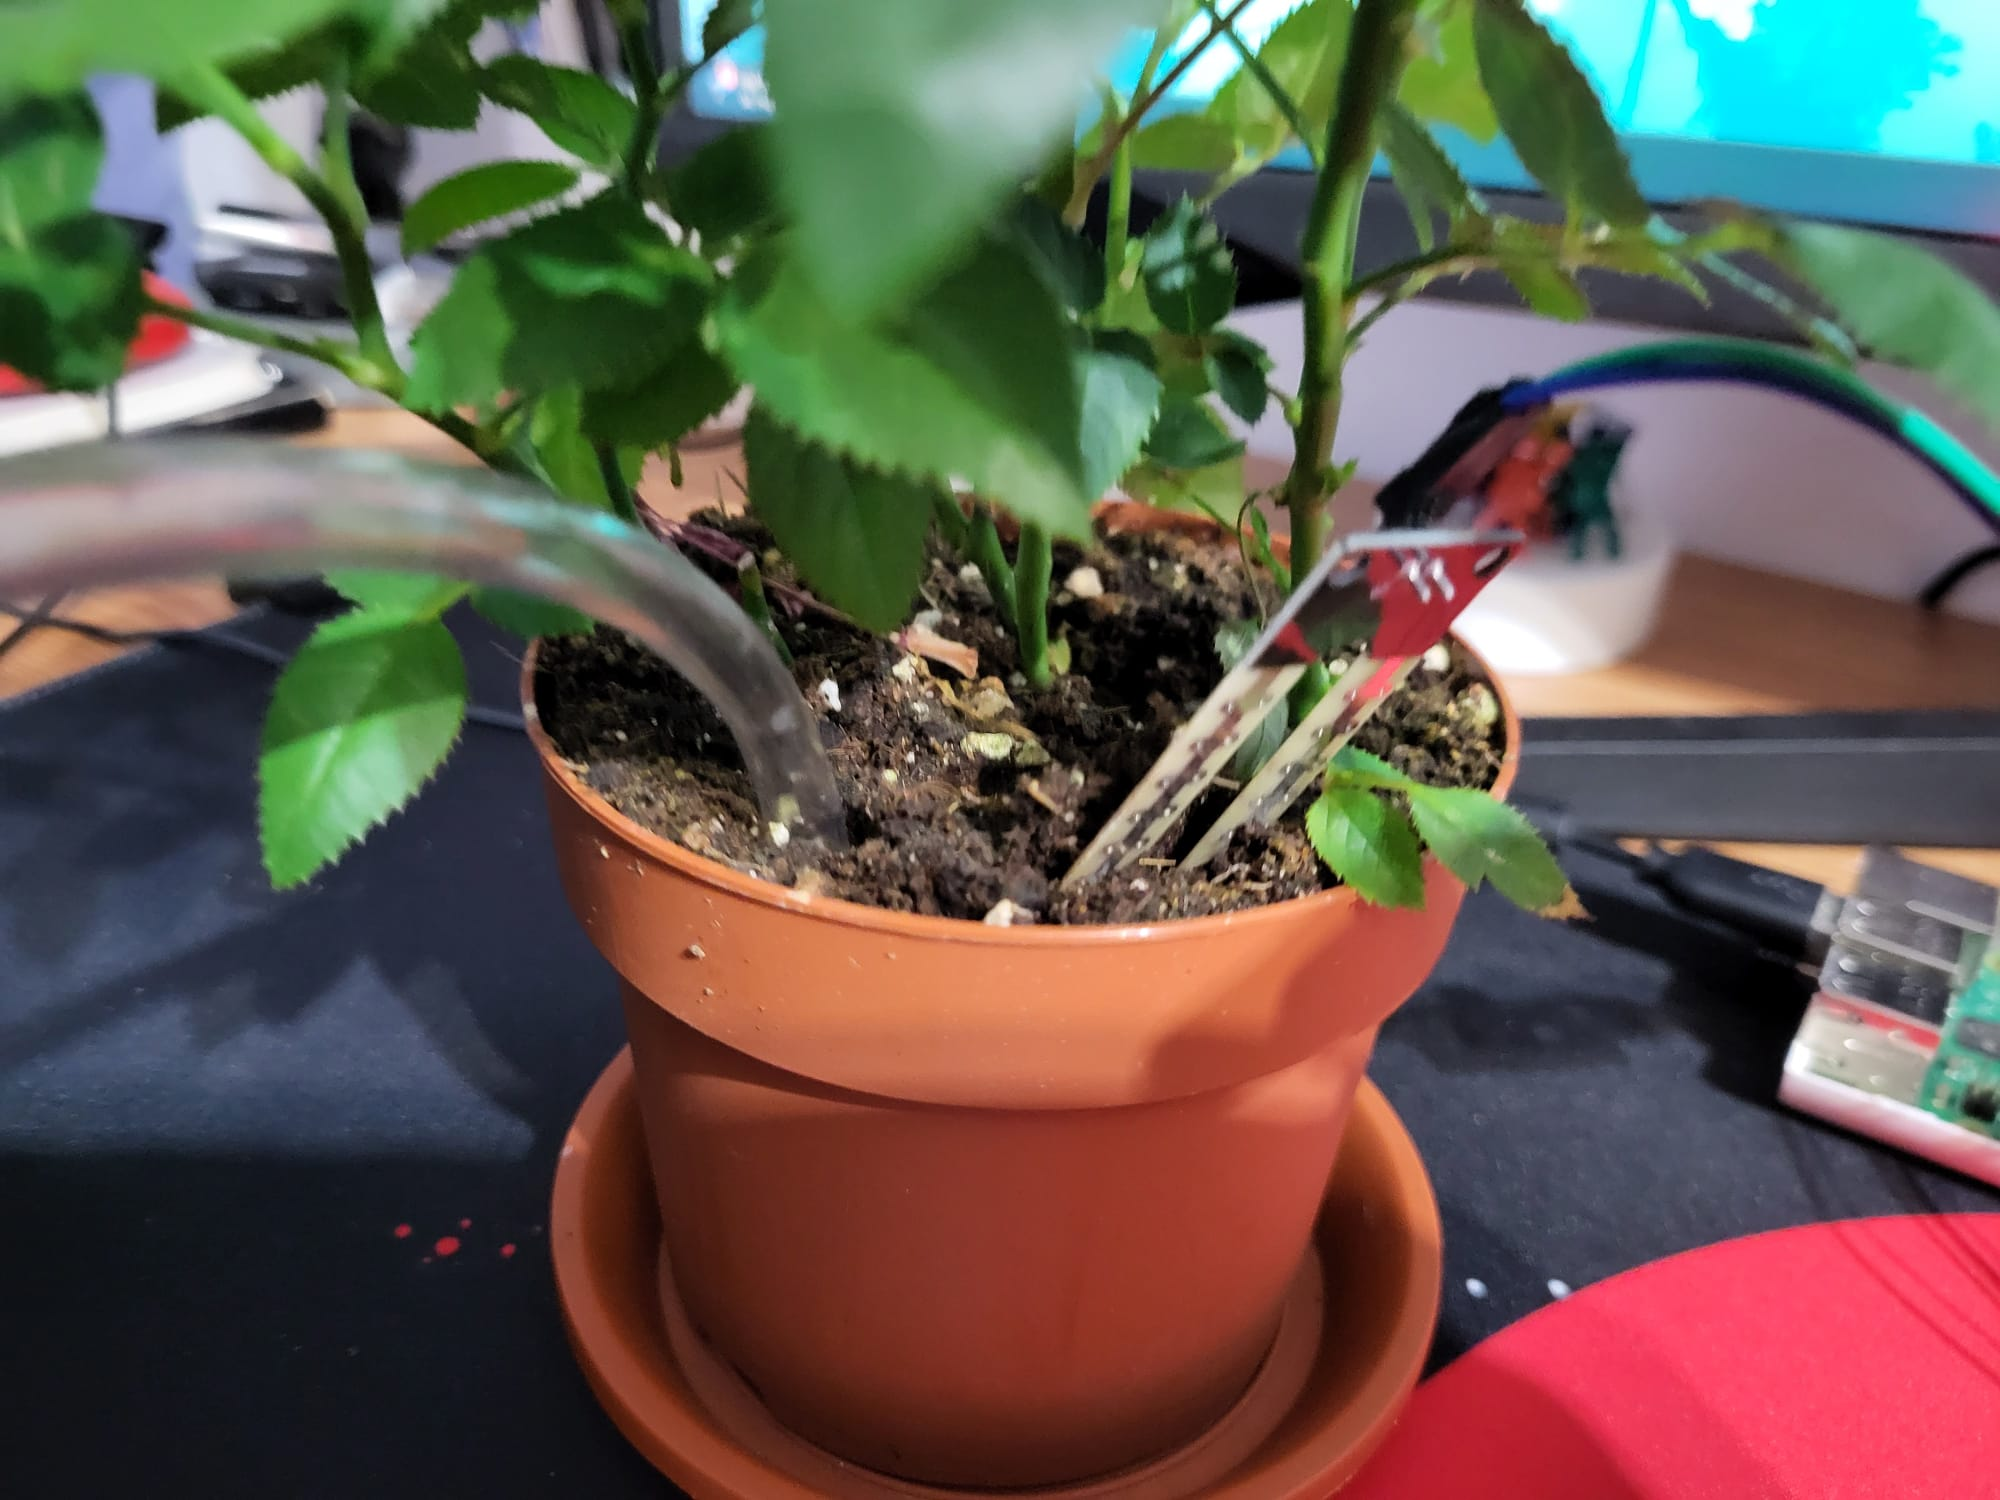
\includegraphics[width=0.53\textwidth]{images/image17.jpeg}
\end{figure} 

\newpage

\begin{figure}[ht]
    \centering
    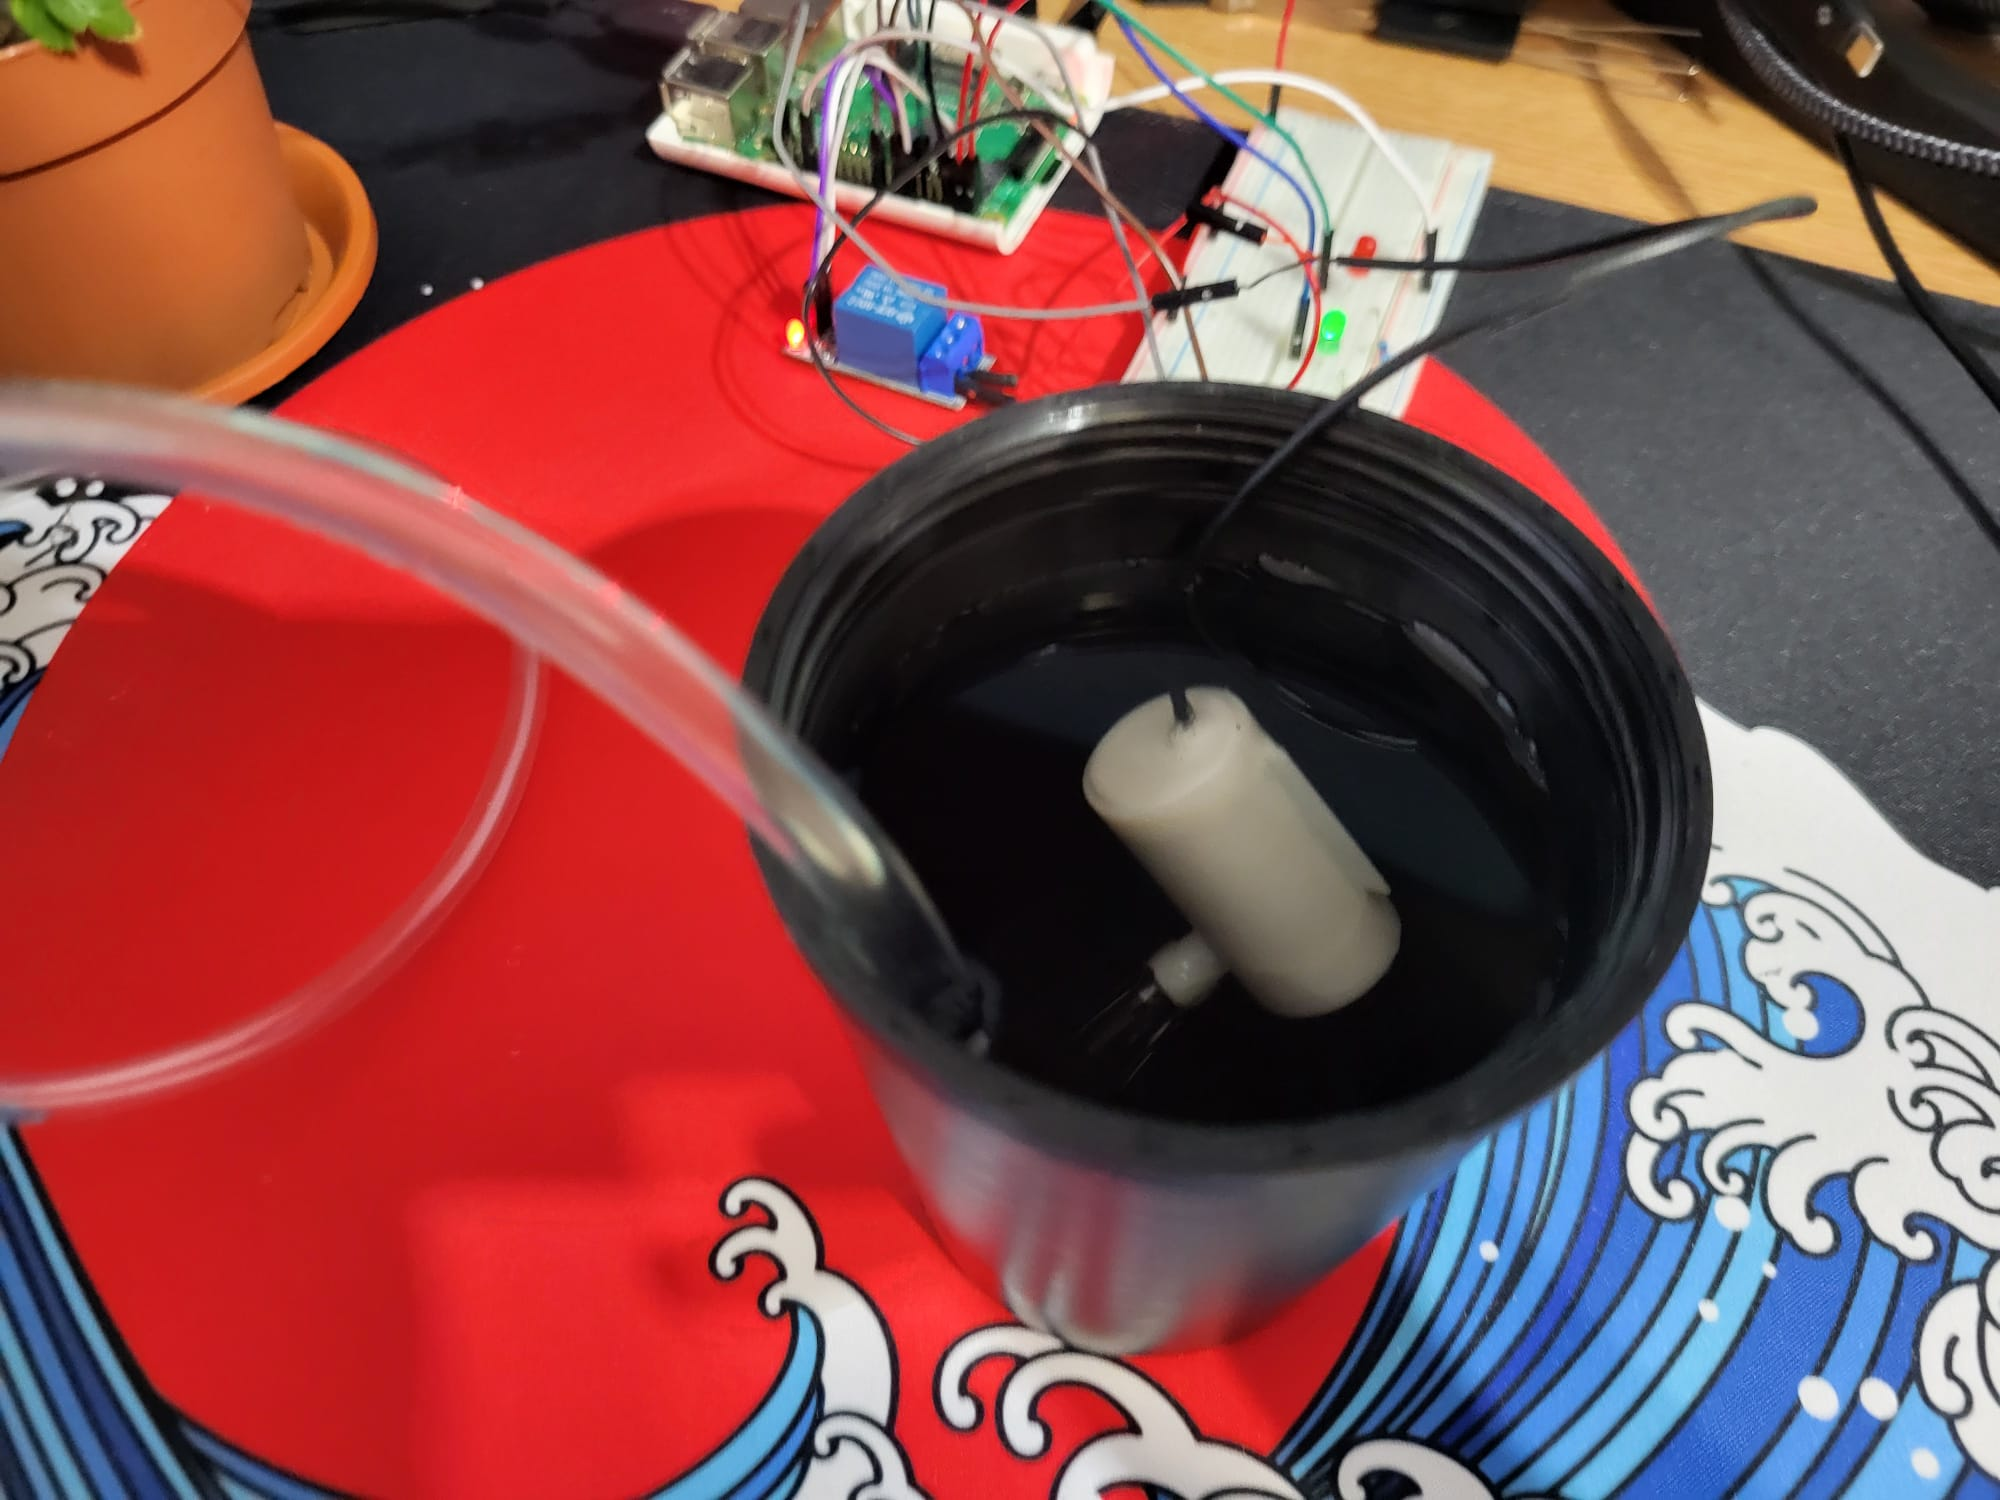
\includegraphics[width=0.55\textwidth]{images/image18.jpeg}
\end{figure} 

\subsection{Flask webpage}

\begin{figure}[ht]
    \centering
    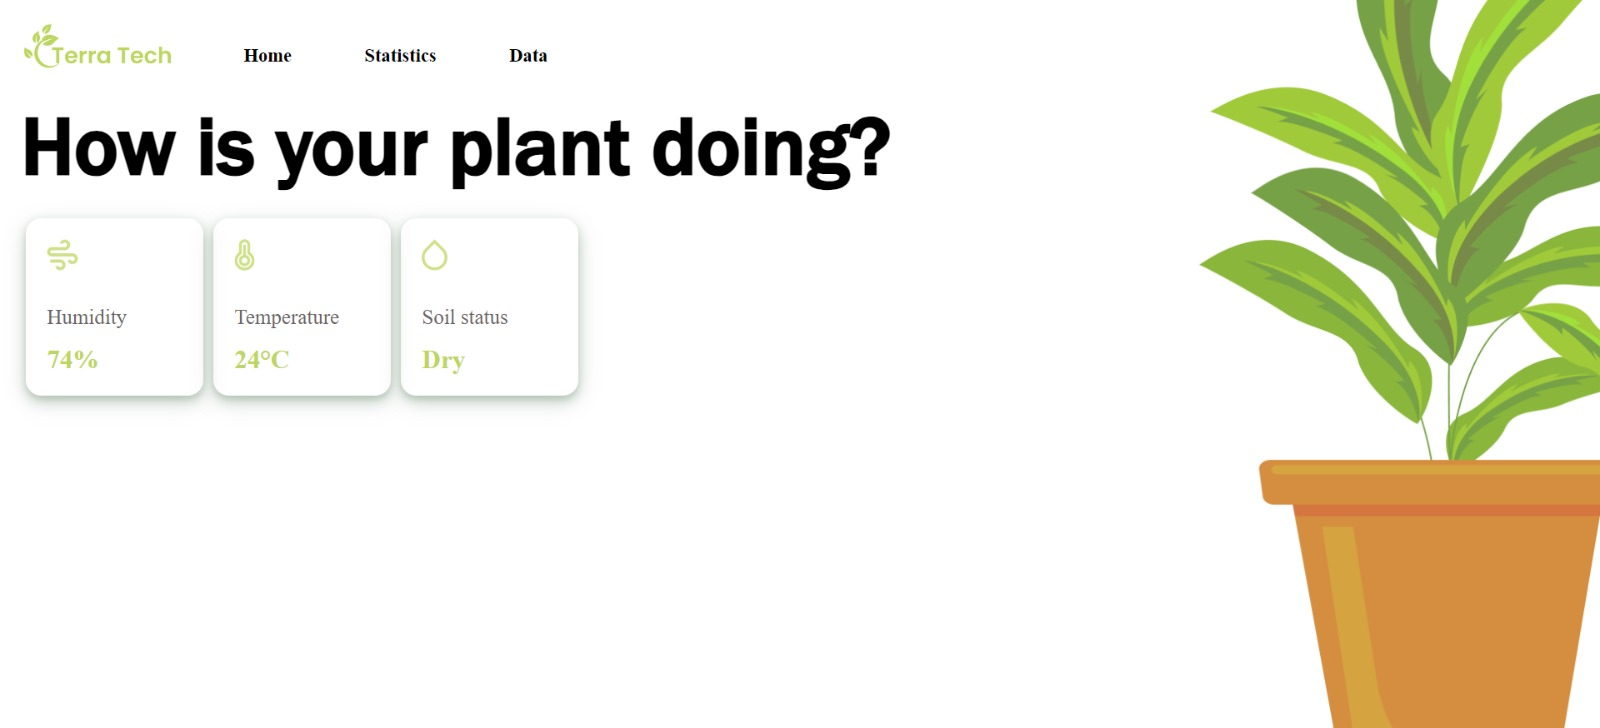
\includegraphics[width=0.8\textwidth]{images/image19.jpeg}
\end{figure}

\begin{figure}[ht]
    \centering
    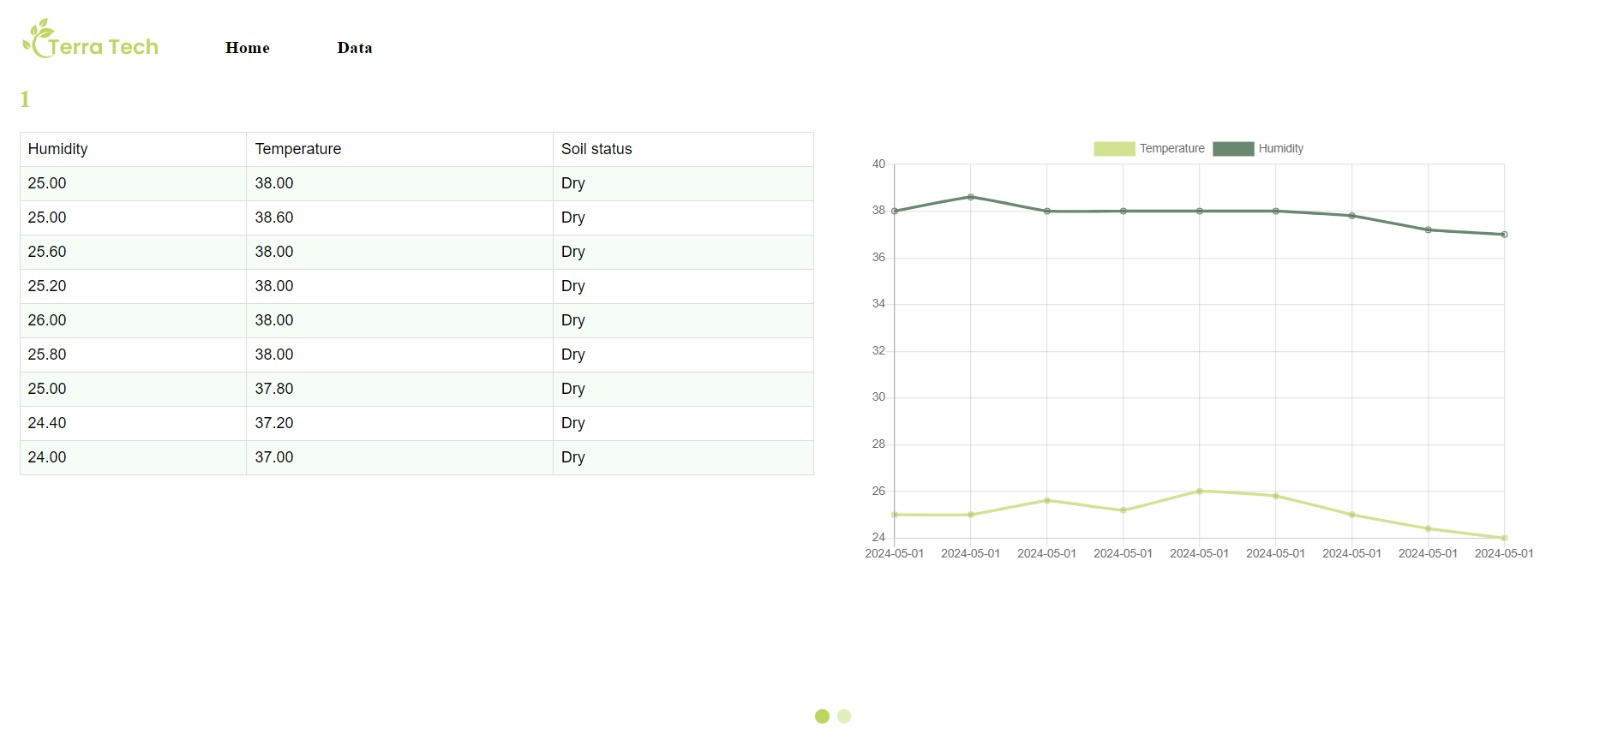
\includegraphics[width=0.9\textwidth]{images/image20.jpeg}
\end{figure}

\newpage

\section{Architecture of the system and subsystems}

\begin{figure}[ht]
    \centering
    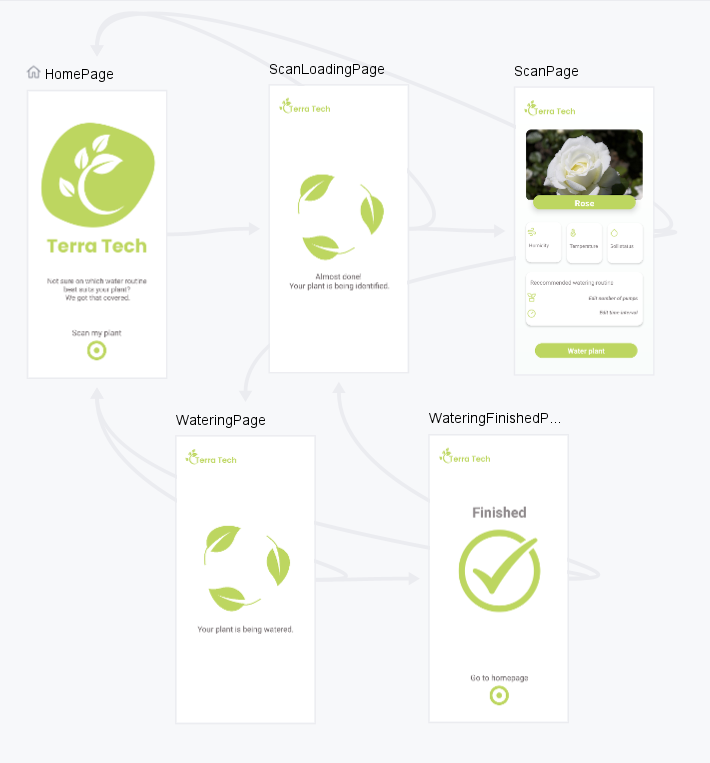
\includegraphics[width=1.1\textwidth]{images/image7.png}
    \caption{Android application flow}
    \label{fig:pic7}
\end{figure} 

\newpage

\section{Short descriptions of technologies used}

\begin{itemize}[leftmargin=2cm]
    \item Java-based Android development
    \item[] The application was developed in Android Studio, using the Android software development kit (SDK). The application code is written in Java, using XML files for layout and styling. \\
    Accessing and running scripts from the RaspberryPi computer is done through Jsch, a pure Java implementation of SSH2. 
    \item Python Flask + Pymssql
    \item[] Flask is a lightweight Python web framework known for its simplicity and versatility, ideal for small to medium-sized projects. \\
    The connection to the RDS database is established through Pymssql, a simple database interface for Python that provides a Python DB-API interface to Microsoft SQL Server.
    \item AWS database
    \item[] Amazon Relational Database Service (Amazon RDS) is a collection of managed services that makes it simple to set up, operate, and scale databases in the cloud. \\
    For database management, Microsoft’s SQL Server Management Studio is used.
    \item Raspberry Pi 3 Model B+
    \item[] 
    The Raspberry Pi 3 Model B+ is a compact single-board computer (SBC) developed by the Raspberry Pi Foundation.\\
    This model was chosen due to its numerous range of ports, especially GPIOS, which is perfect for reading data from our sensor, and sending values to the water pump actuator in order to turn it on/off.
    \item Tensorflow AI model
    \item[] TensorFlow is a powerful machine learning framework developed by Google. \\
    This project's model is trained on five species of flowers: daisies, dandelions, roses, sunflowers and tulips.
\end{itemize}

\newpage 
\section{Code examples and code descriptions}

\subsection{Raspberrypi scripts}
\begin{figure}[ht]
    \centering
    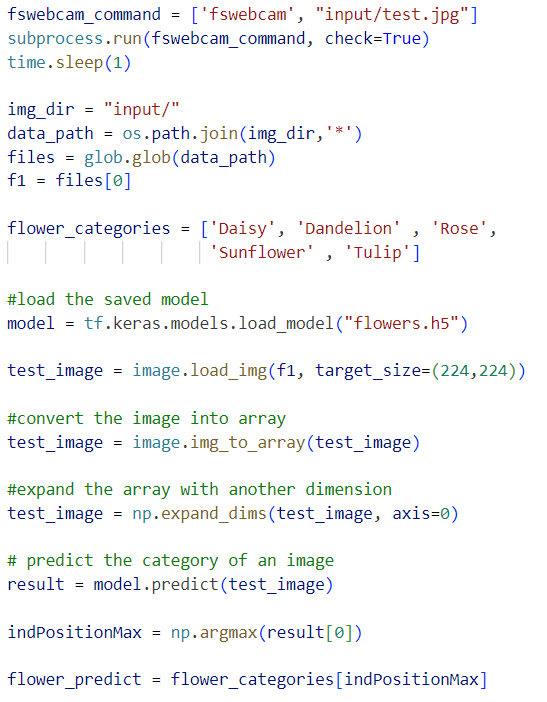
\includegraphics[width=0.75\textwidth]{images/image12.png}
    \caption{An image is captured through the webcam and saved in the input directory. A pre-trained AI model is loaded and ran on the captured image. The result is given by the model.predict function call.}
    \label{fig:pic12}
\end{figure} 

\newpage

\begin{figure}[ht]
    \centering
    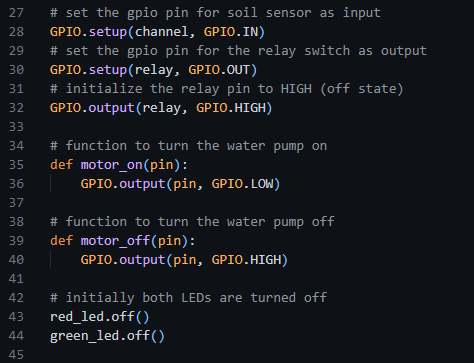
\includegraphics[width=0.7\textwidth]{images/image10.png}
    \caption{The GPIO for the soil sensor is set as input because information is taken from it and is used in the code. For 5v Relay the GPIO is set on output in order to send the signal from the code to it and then to the water pump.
    The initial value for 5V Relay is High meaning the off state for it (the relay is turned off). Both LEDs are initially turned off.}
    \label{fig:pic10}
\end{figure} 
    
\begin{figure}[ht]
    \centering
    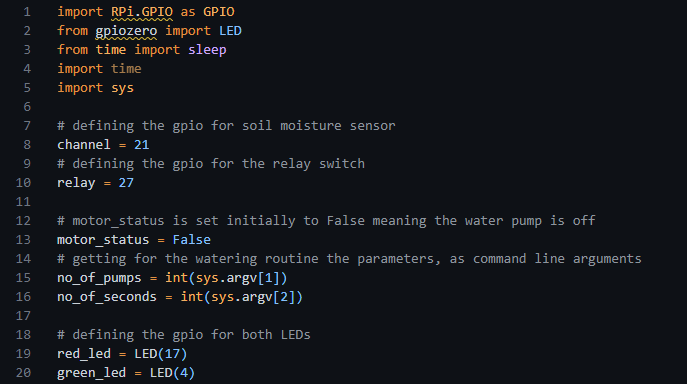
\includegraphics[width=0.725\textwidth]{images/image9.png}
    \caption{Because the soil sensor is connected to GPIO21 and the 5V Relay to GPIO27 they are defined in 2 variables.
    The LEDs are connected to GPIO17 and GPIO4 so they are also taken and stored into 2 variables, one for each led.}
    \label{fig:pic9}

\end{figure} 

\newpage

\subsection{Android application}

\begin{figure}[ht]
    \centering
    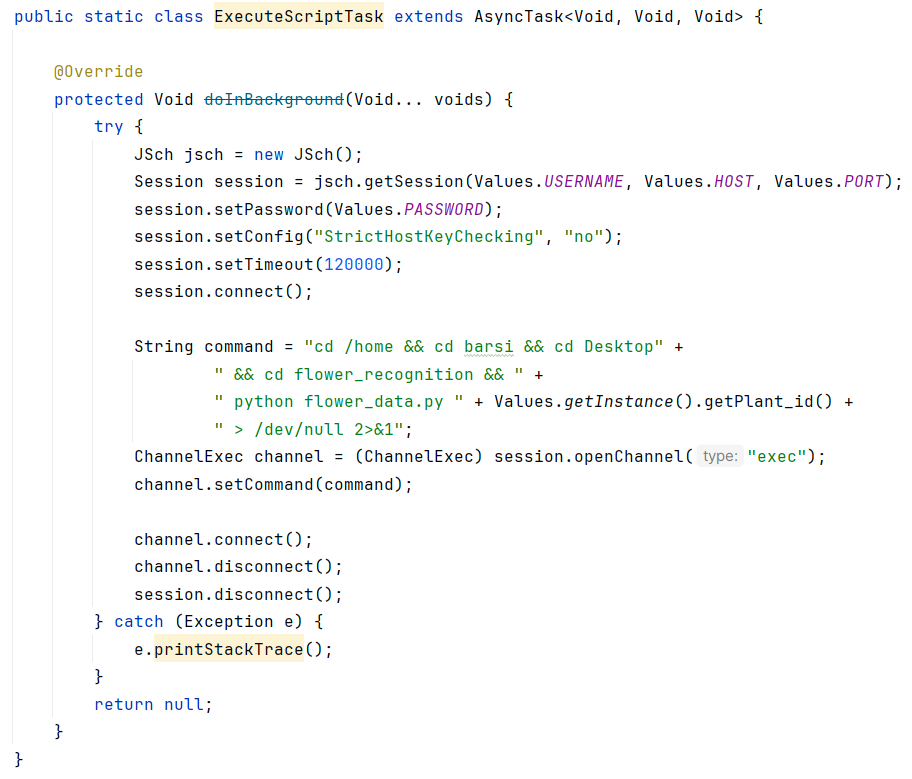
\includegraphics[width=0.9\textwidth]{images/image4.png}
    \caption{Commands are sent to the RaspberryPi from the application via ssh (JSch is the Java implementation of SSH2 that allows connection to an SSH server). \\
    The execution of the commands opens the directory of the Python script and executes it with a command line argument.}
    \label{fig:pic1}
\end{figure}  

\newpage

\begin{figure}[ht]
    \centering
    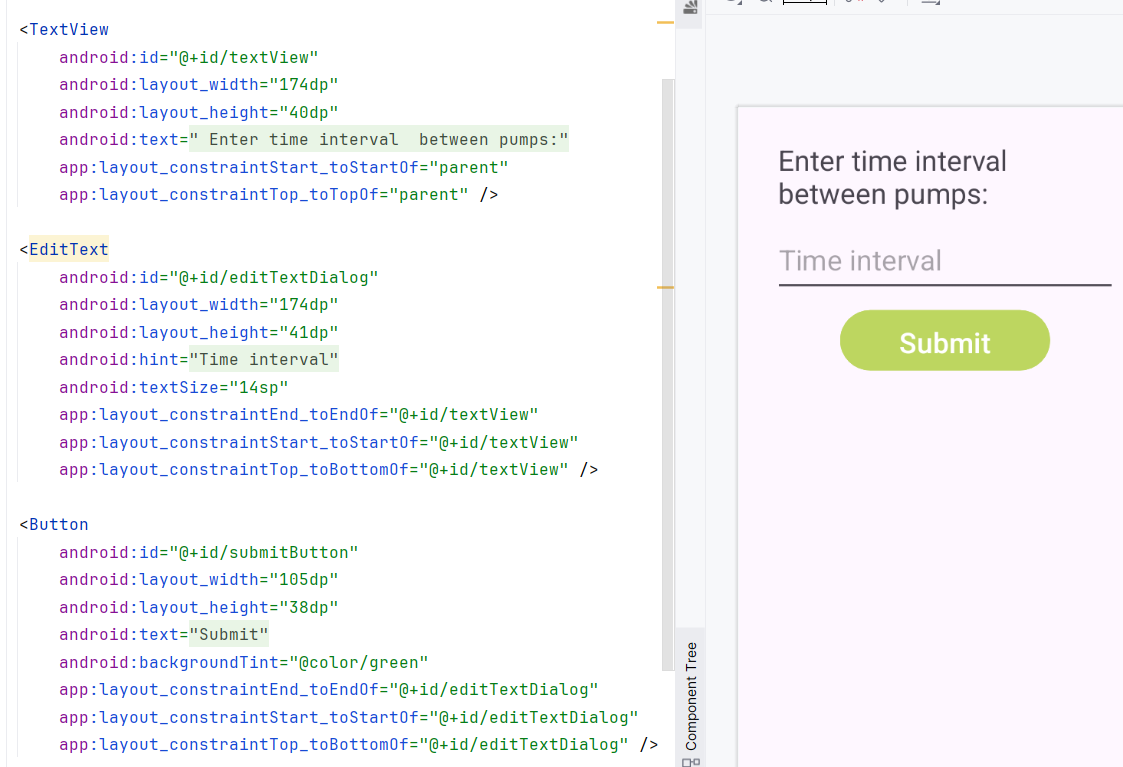
\includegraphics[width=0.87\textwidth]{images/image1.png}
    \caption{Snippet of an xml layout file for one of the popups that lets the user edit the time interval between pumps.}
    \label{fig:pic3}
\end{figure} 


\begin{figure}[ht]
    \centering
    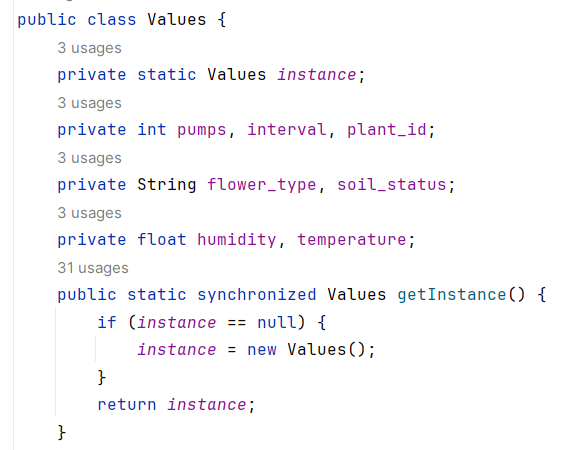
\includegraphics[width=0.56\textwidth]{images/image3.png}
    \caption{For variables that are used and modified throughout the app in multiple pages, a public singleton class is used; the values are accessed and modified via getters and setters.}
    \label{fig:pic2}
\end{figure} 


\newpage

\subsection{Flask website}

\begin{figure}[ht]
    \centering
    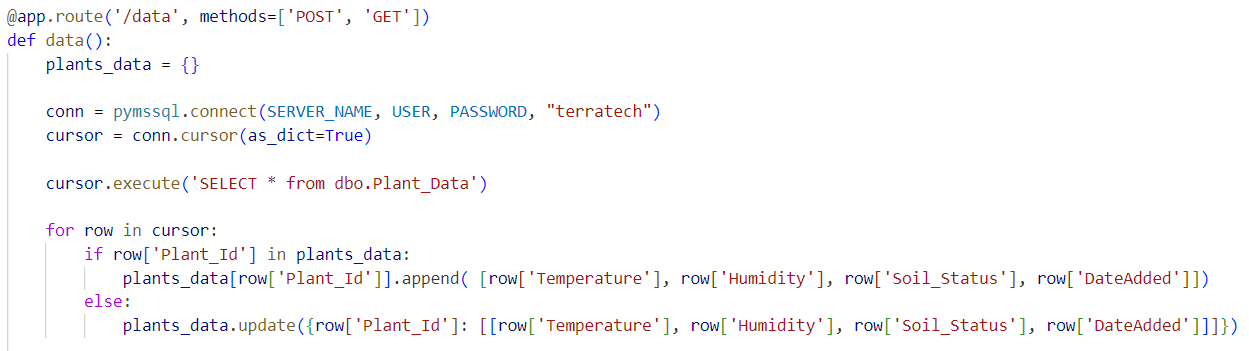
\includegraphics[width=1\textwidth]{images/image2.png}
    \caption{Communication with the server is done with Pymssql (a simple database interface for Python that builds on top of FreeTDS to provide a Python DB-API interface to Microsoft SQL Server). \\
    For the page displaying the data and the graphs, the data is read from the database and separated by plant id. }
    \label{fig:pic4}
\end{figure} 

\begin{figure}[ht]
    \centering
    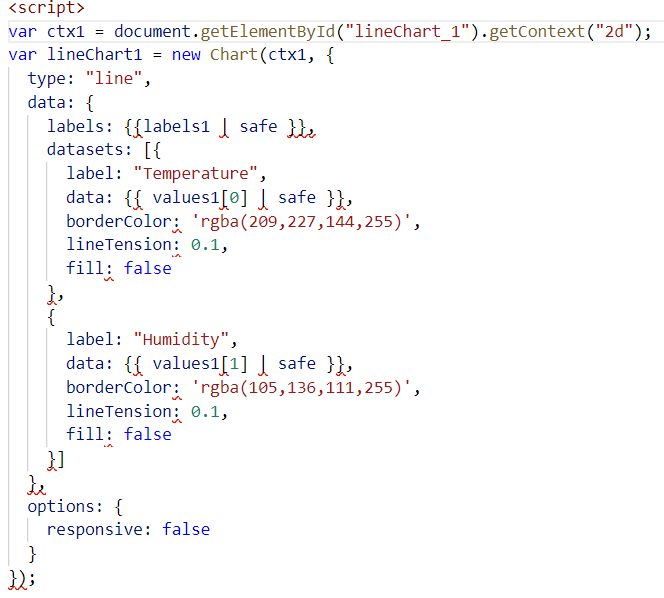
\includegraphics[width=0.67\textwidth]{images/image6.png}
    \caption{Each plant (distinguishable by plant id) has its own page where the data is displayed in both table and graph form. The Javascript code above is for the graph, specifying what the X axis (labels) and Y axis (datasets - can have multiple sets of data) are portraying. }
    \label{fig:pic4}
\end{figure} 

\newpage

\section{Future work}

\begin{itemize}[leftmargin=2cm]
\item Expanding the knowledge of the AI model to be able to distinguish between more species of plants;
\item Researching watering recommendations for plants so that the app can be more accurate and effective;
\item Expanding the use of AI to detect pests/diseases that the plants may have;
\item Allowing users to login into the app and website so they only receive data about their plants, and are able to add their plants into the virtual “garden” living in our databases;
\item Use more sensors to monitor the water level for the pump and notify the user when the water in the pump is running low, by sending an alert on the app;
\item Adding an ADC to extract precise data from the soil moisture sensor.
\end{itemize}

\nocite{*} % Include all entries from the .bib file


\bibliographystyle{plainnat} % Specify the bibliography style
\bibliography{references}


\end{document}